\begin{frame}
  \frametitle{Effective multiplication factor for full-core \gls{MSBR} model }
    \begin{columns}
    \column[t]{7cm}
   \vspace{-0.35in}
  \begin{figure}[t]
   \hspace*{-0.2in}
   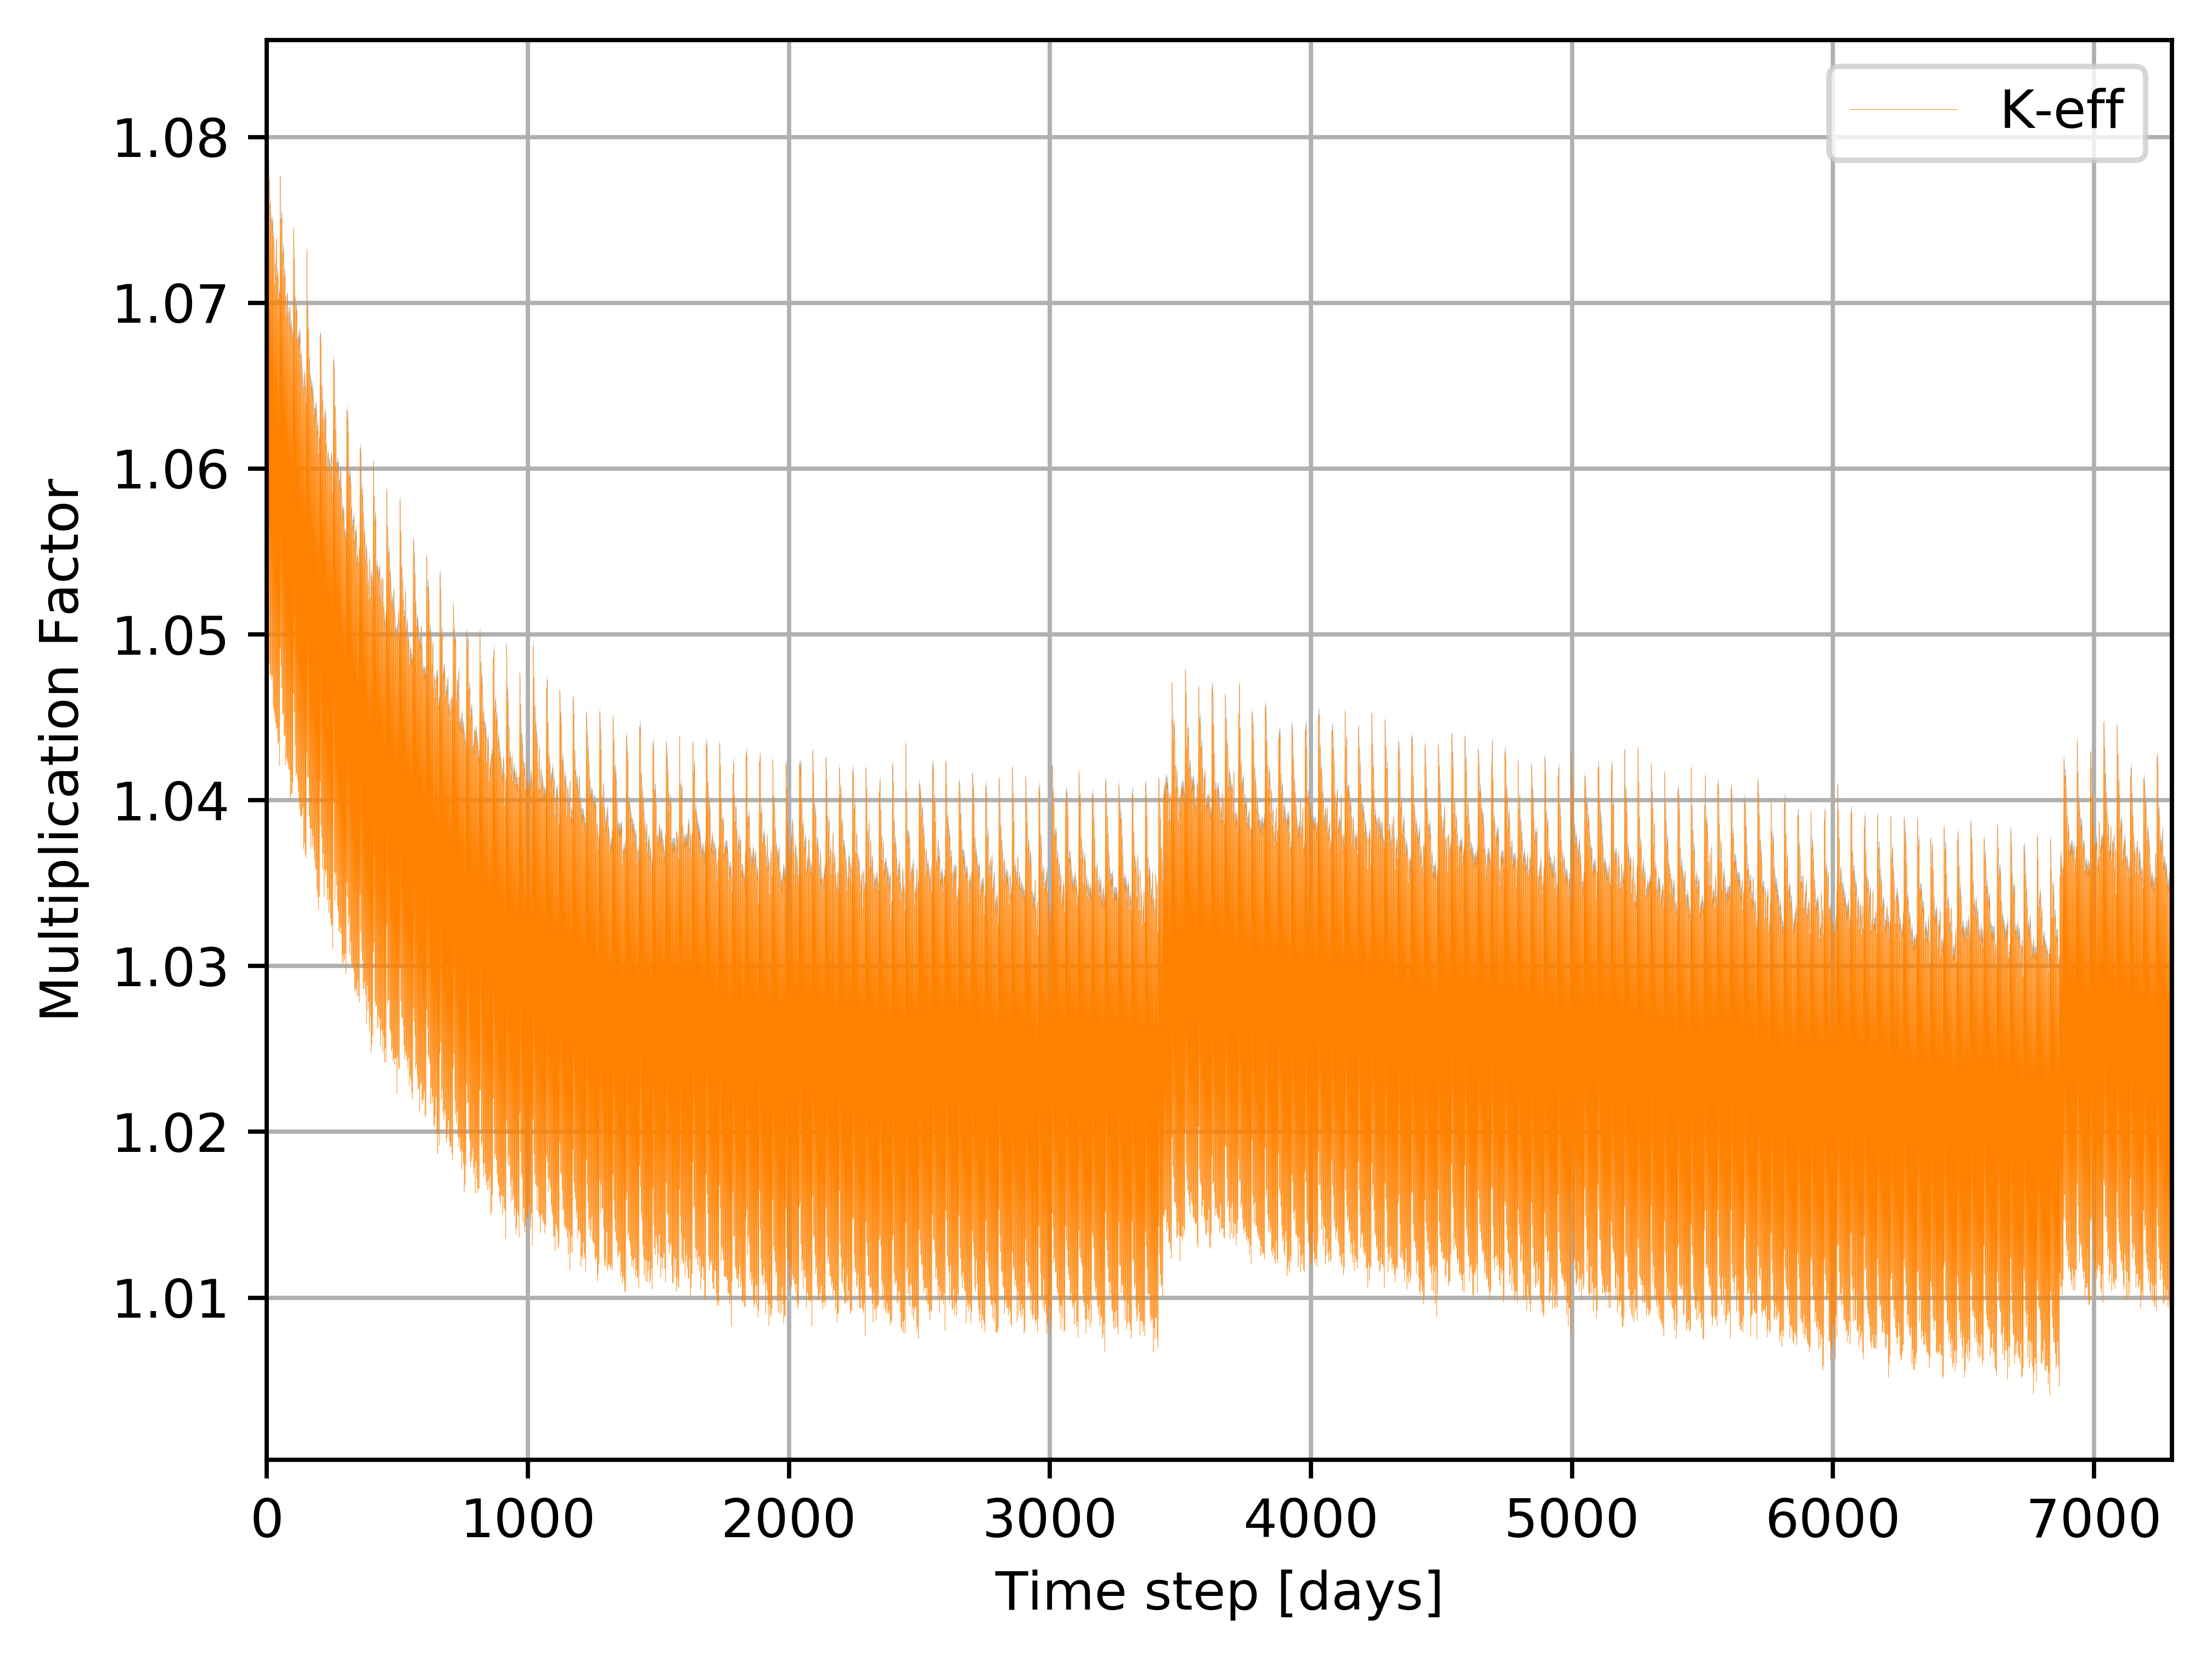
\includegraphics[height=0.75\textheight]{./images/keff.png}
   \vspace{-0.05in}
   \caption{$k_{eff}$ during a 20 years depletion simulation.}
    \end{figure}

    \column[t]{4.5cm}
       \begin{itemize}
	        \item Strong absorbers ($^{233}$Th,$^{234}$U) accumulating in the core
   		\item Fissile materials other than $^{233}$U are bred into the core ($^{235}$U, $^{239}$Pu)
   		\item The multiplication factor stabilizes after approximately 6 years
       \end{itemize}
     \end{columns}
\end{frame}

\begin{frame}
  \frametitle{Power and breeding distribution}
    \begin{columns}
    \column[t]{6cm}
  \begin{figure}[t]
   \vspace{-0.25in}
   \hspace*{-0.15in}
   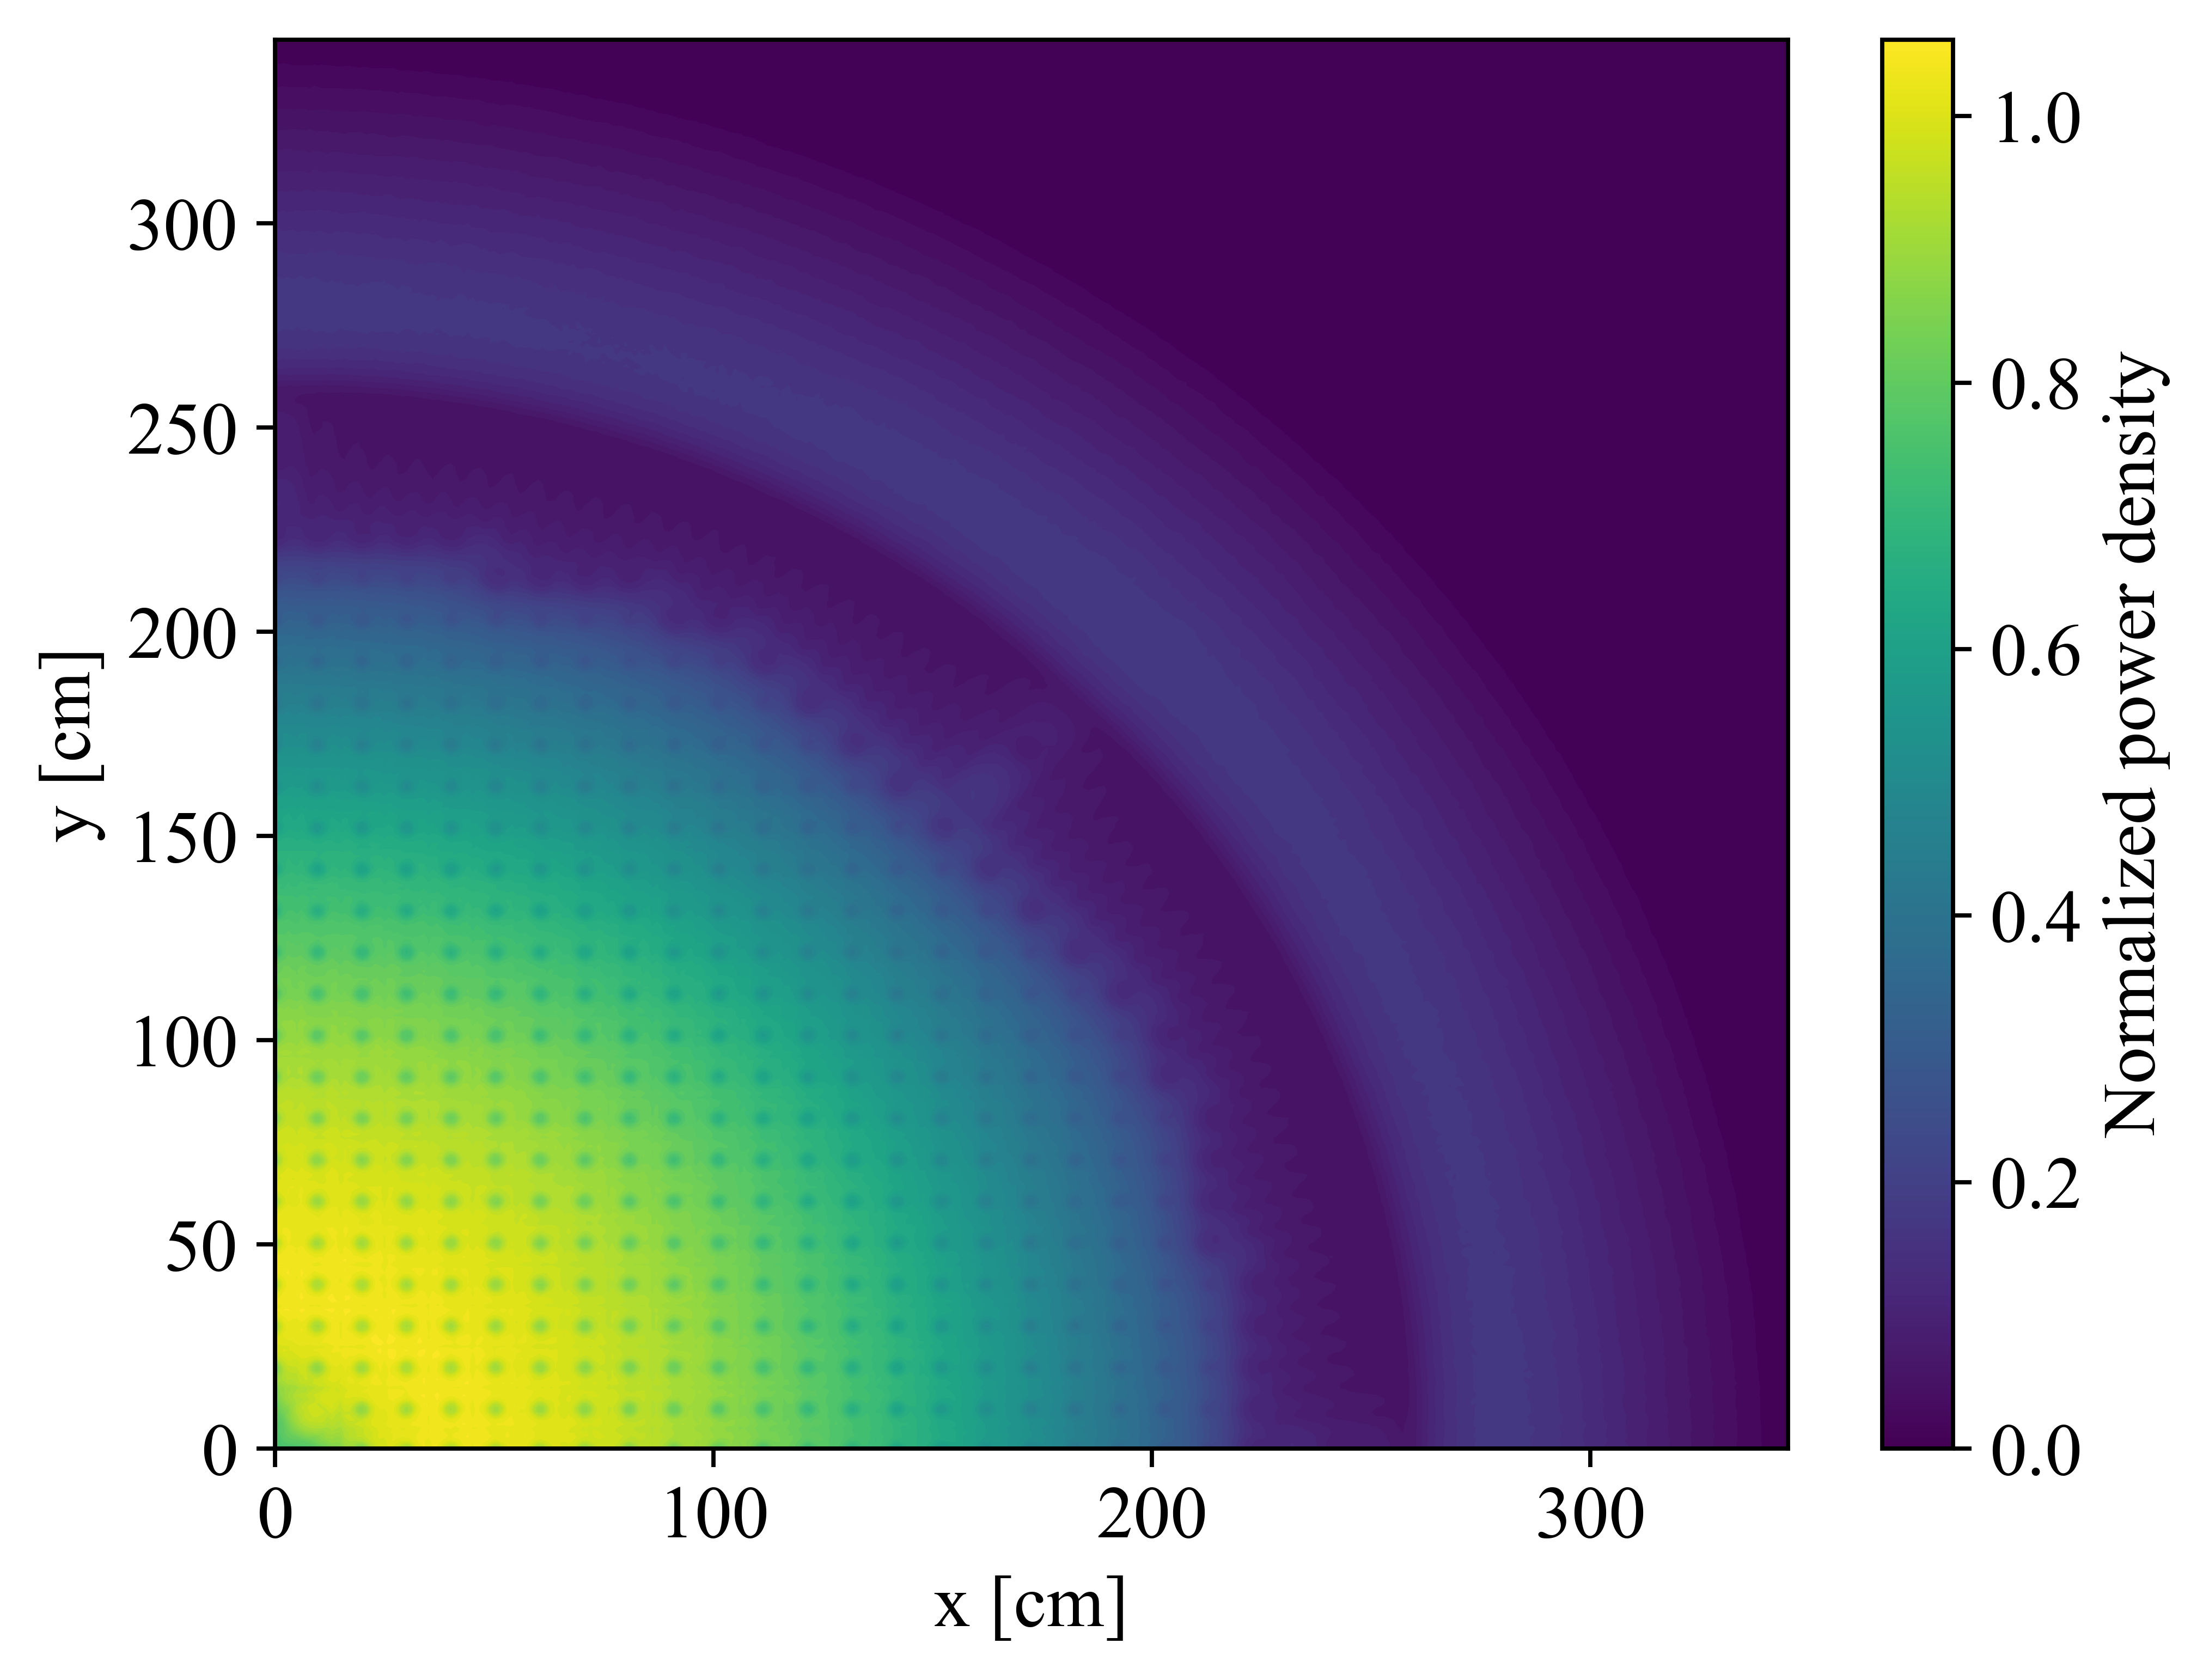
\includegraphics[height=0.6\textheight]{./images/power_distribution.png}
   \vspace{-0.1in}
   \caption{Normalized power density}
    \end{figure}

    \column[t]{6cm}
  \begin{figure}[t]
   \vspace{-0.25in}
	\hspace*{-0.05in}
   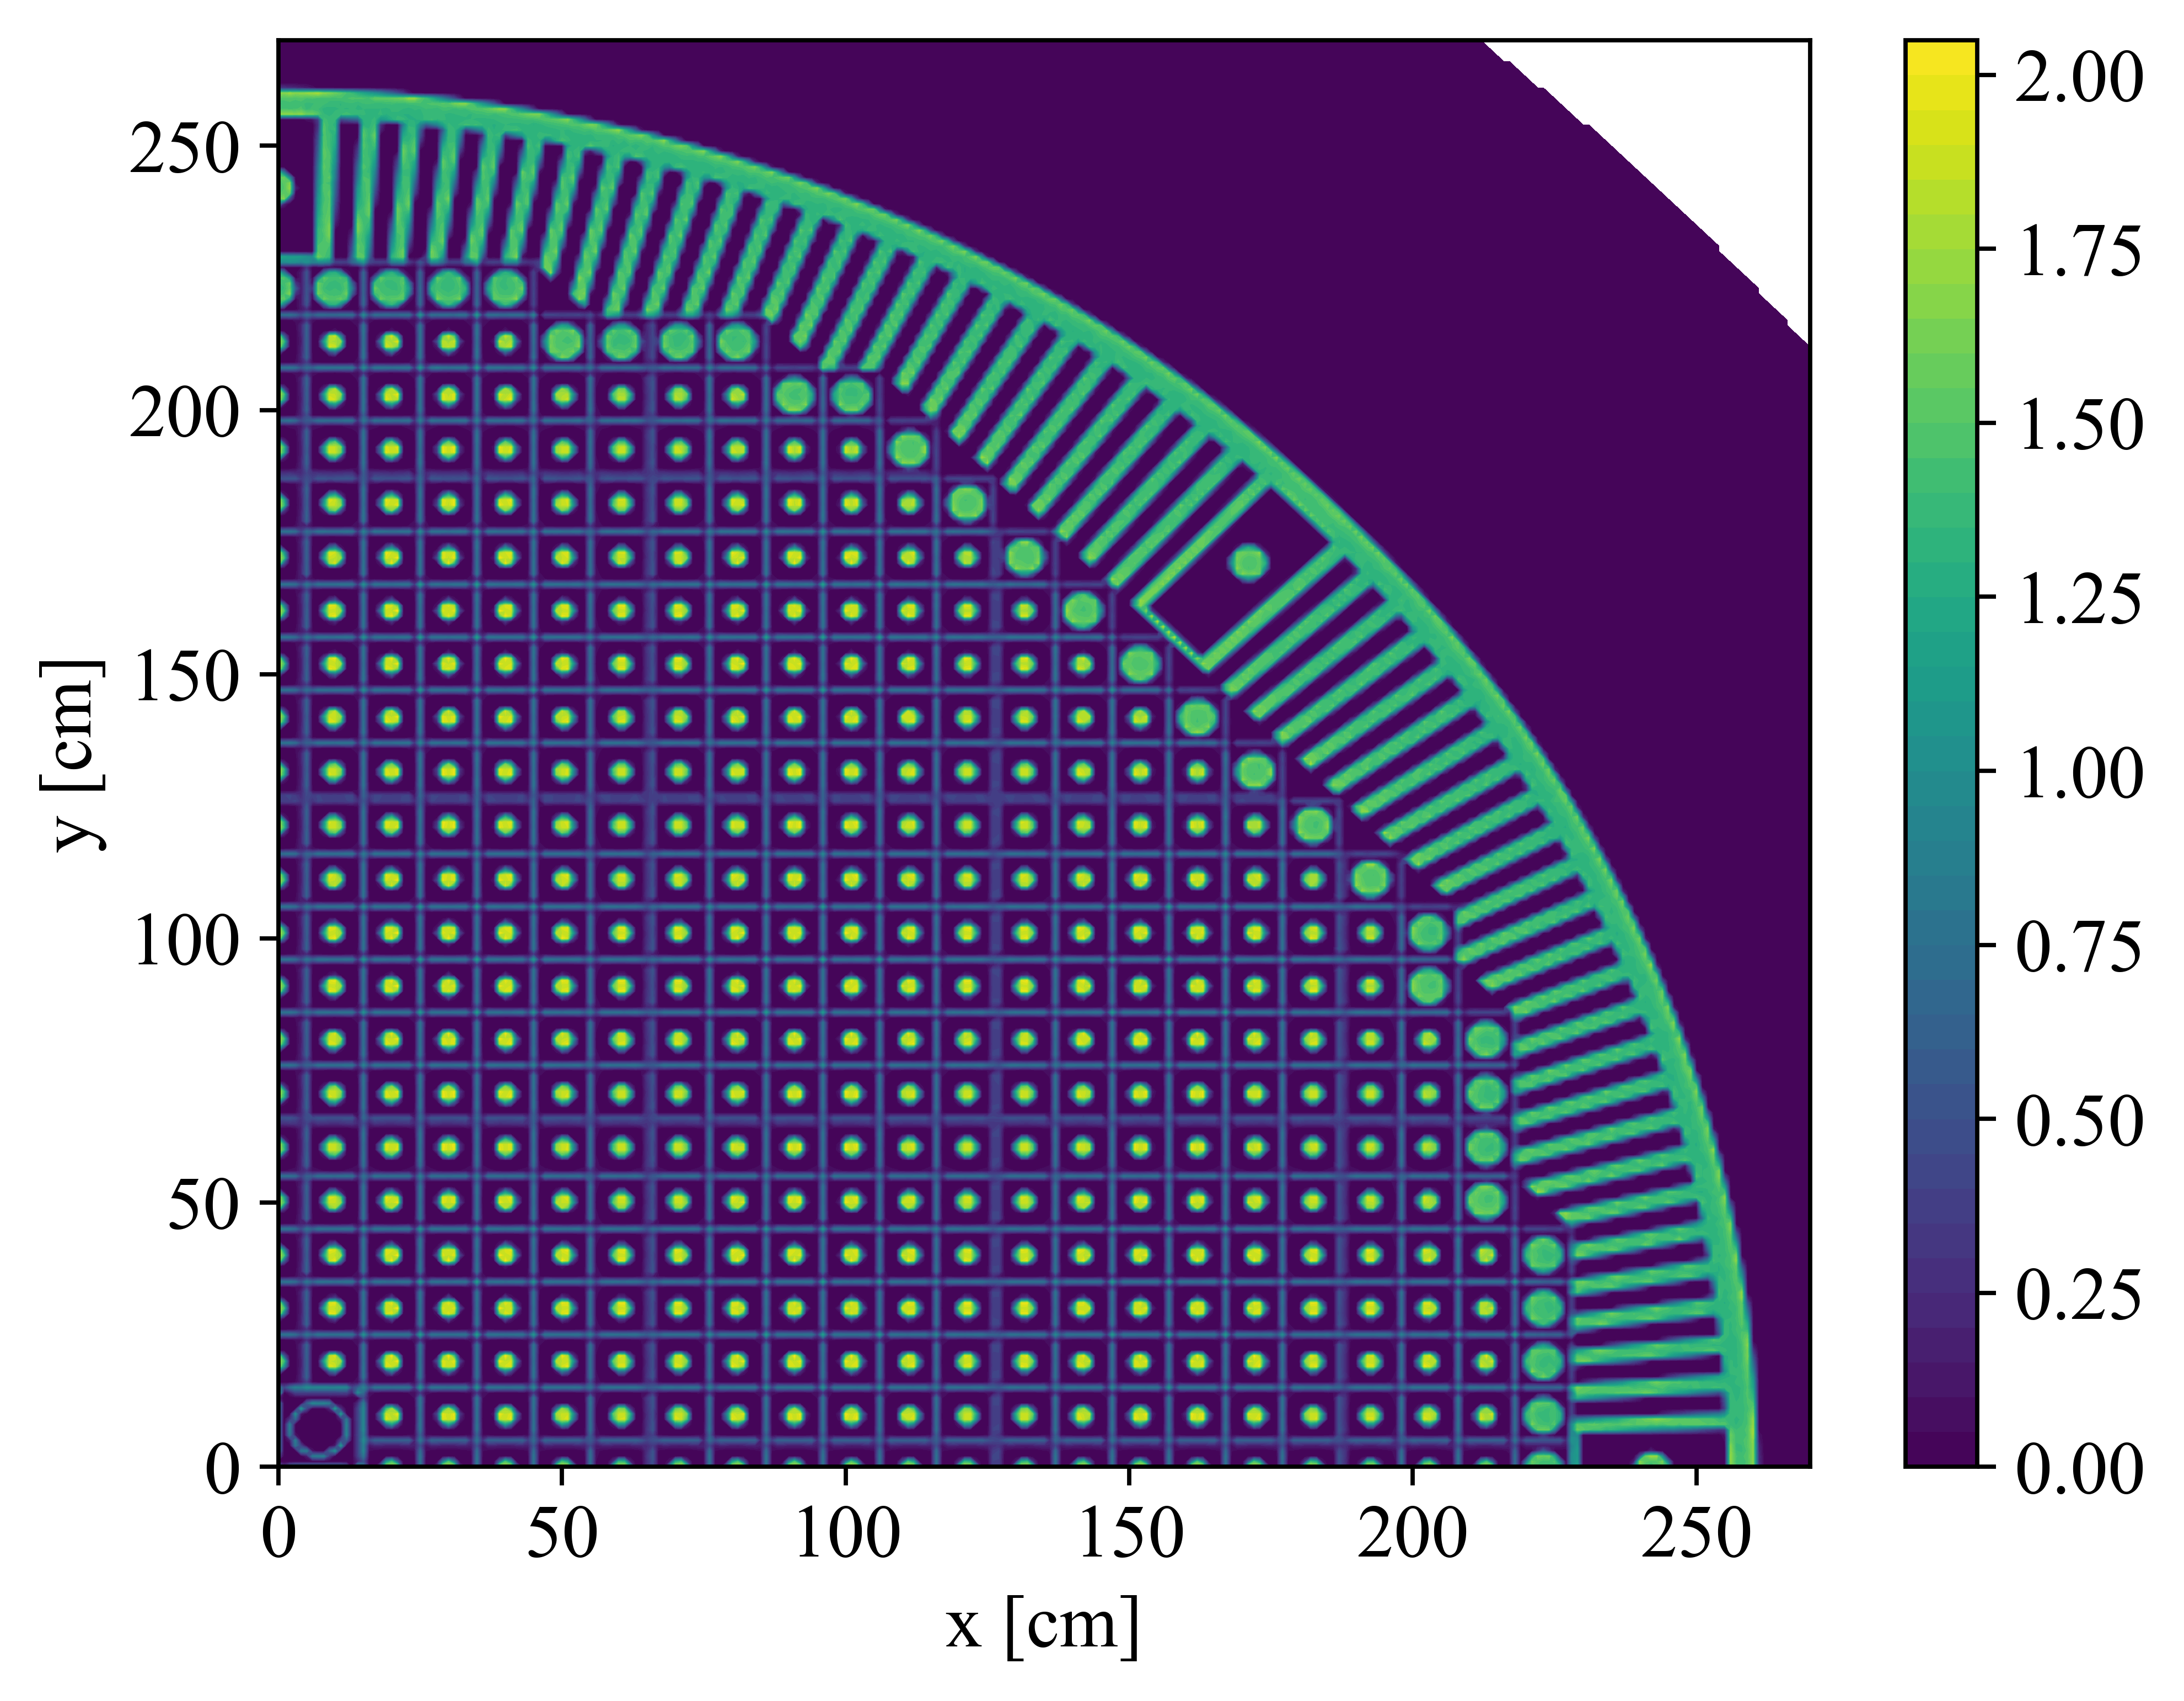
\includegraphics[height=0.6\textheight]{./images/breeding_distribution.png}
   \vspace{-0.1in}
   \caption{$^{232}$Th neutron capture reaction rate normalized by total flux}
    \end{figure}

     \end{columns}
\end{frame}

\begin{frame}
  \frametitle{$^{232}$Th refill rate}
    \begin{columns}
    \column[t]{7cm}
   \vspace{-0.35in}
  \begin{figure}[t]
   \hspace*{-0.2in}
   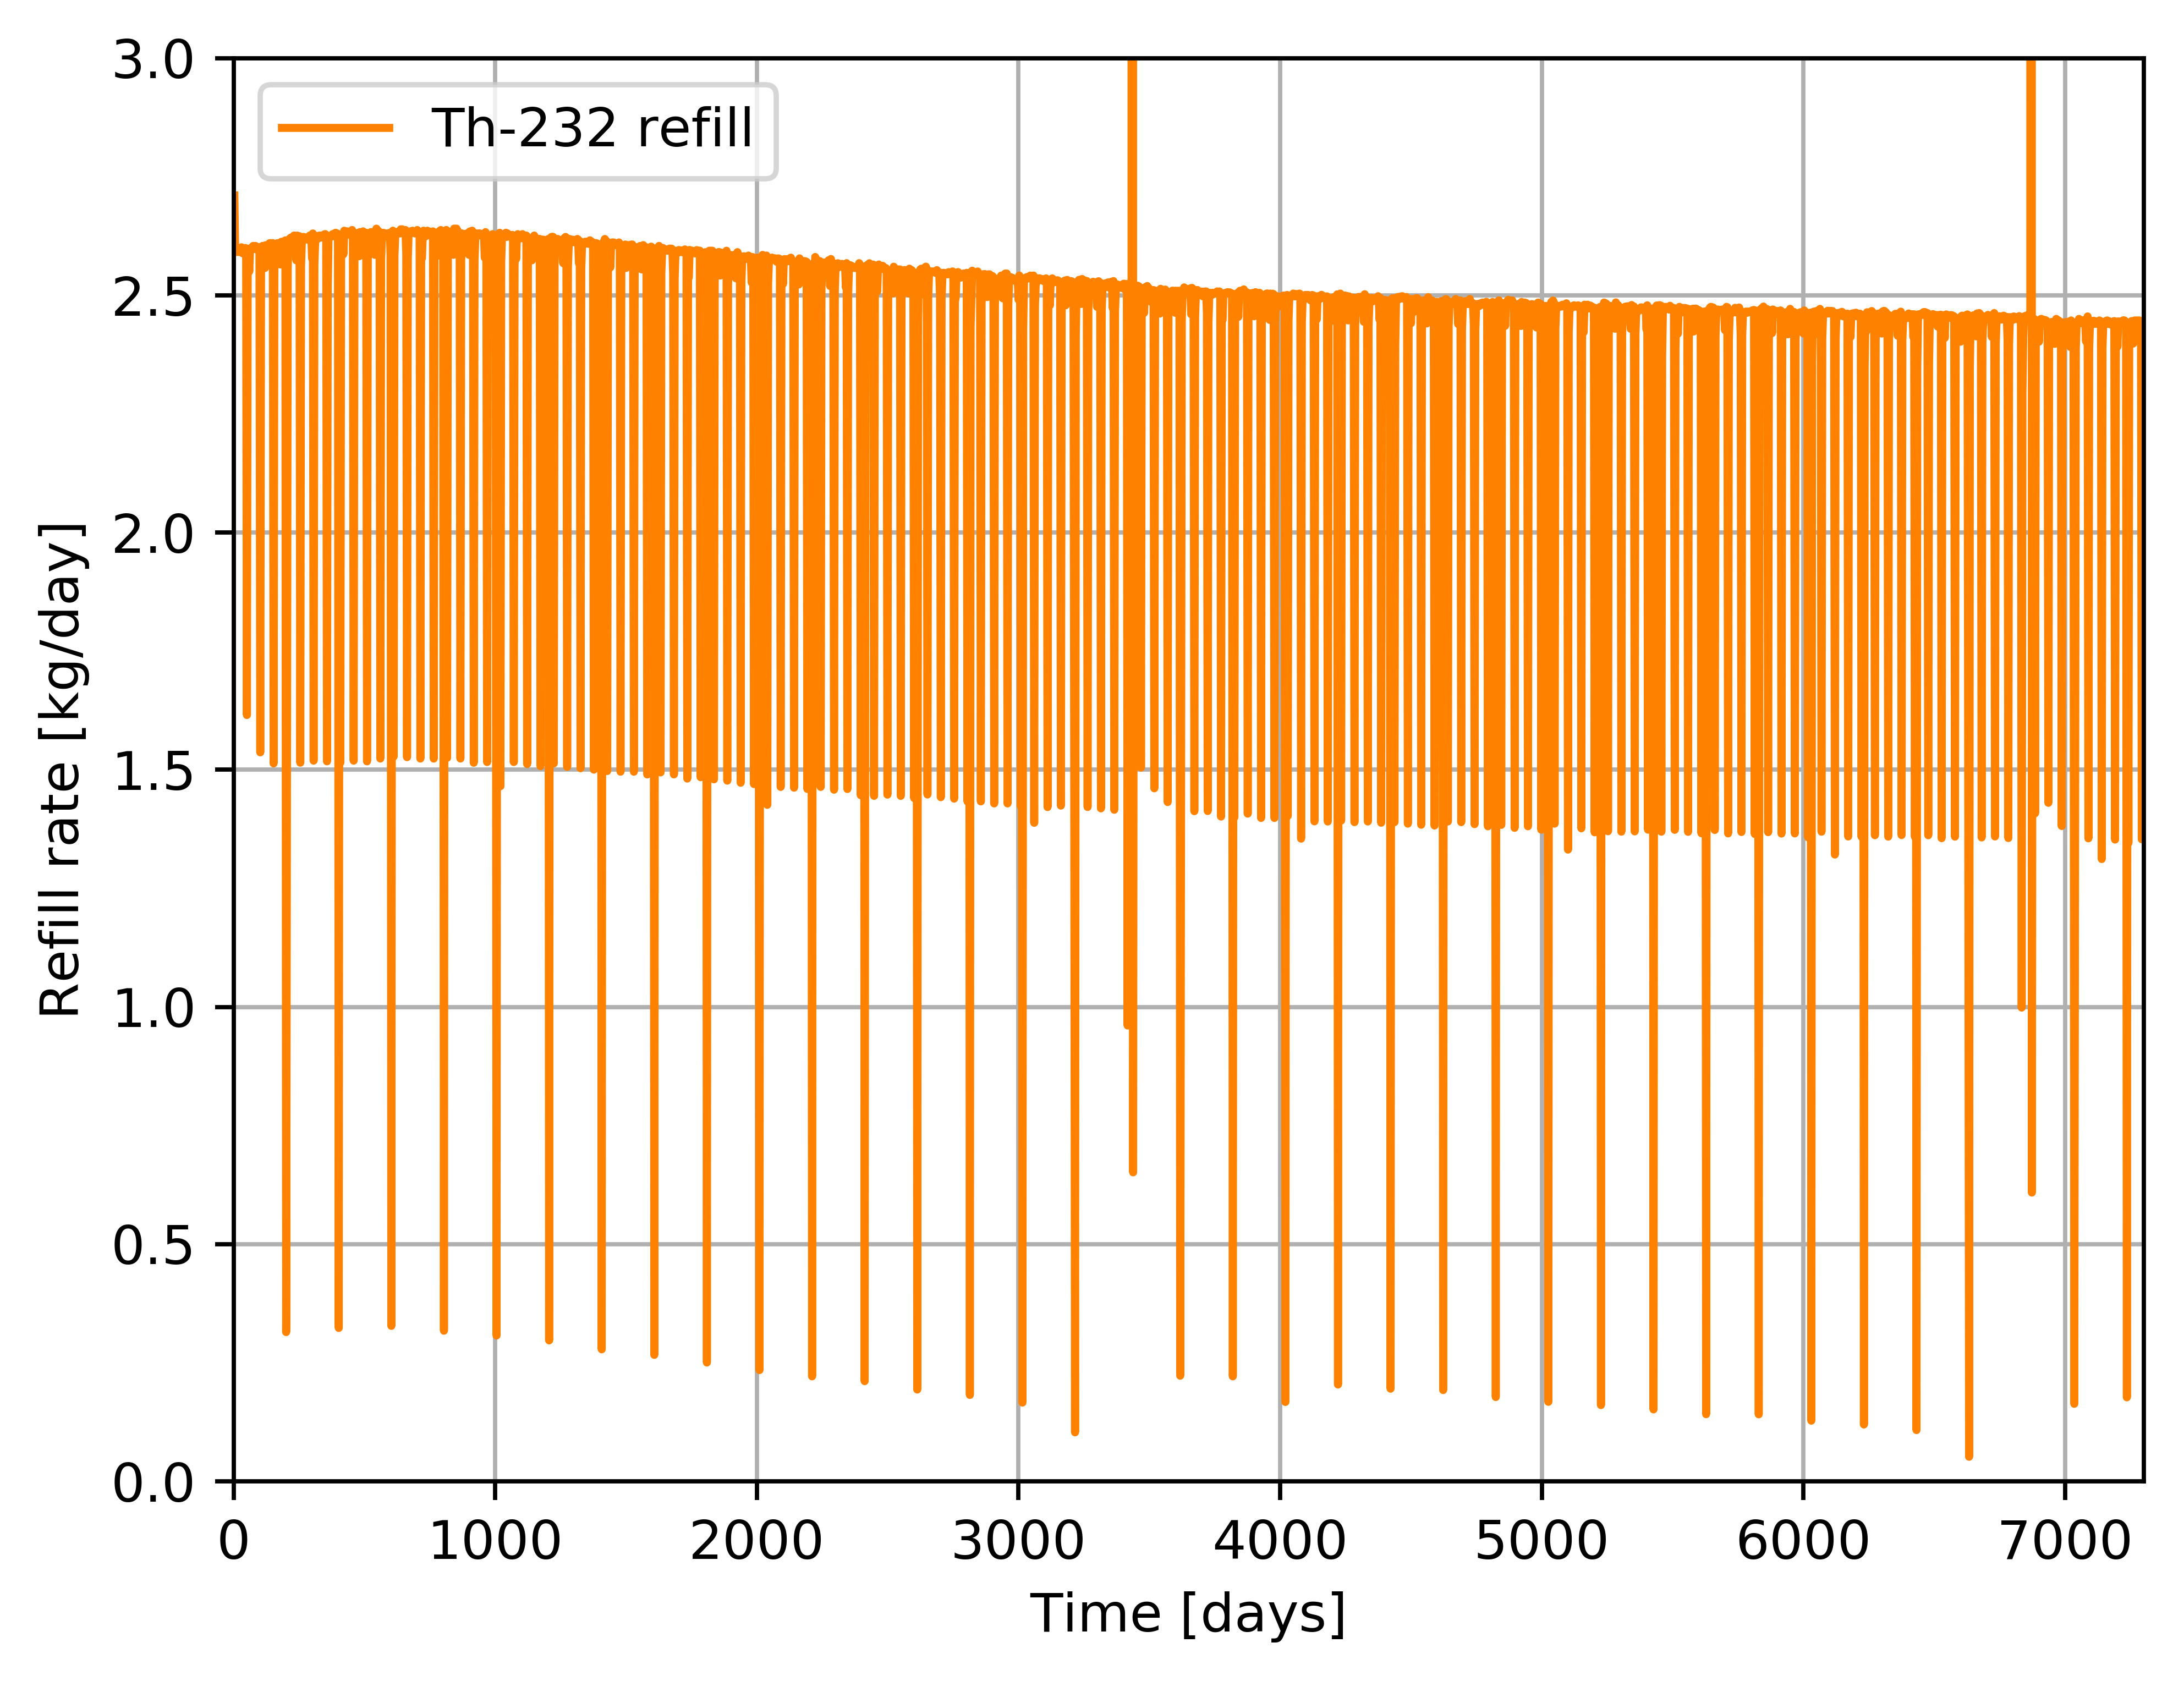
\includegraphics[height=0.75\textheight]{./images/Th_refill_rate.png}
   \vspace{-0.05in}
   \caption{$^{232}$Th feed rate over 20 years of \gls{MSBR} operation}
    \end{figure}

    \column[t]{4.5cm}
       \begin{itemize}
	        \item Fluctuation due to batch-wise removal of strong absorbers
   		\item Feed rate varies due to neutron energy spectrum evolution
   		\item $^{232}$Th consumption is 100 g/GWh$_e$
       \end{itemize}
     \end{columns}
\end{frame}

\begin{frame}
  \frametitle{Multiphysics simulation results (2D)}
  \begin{figure}
   \vspace{-0.05in}
   \hspace*{-0.15in}
   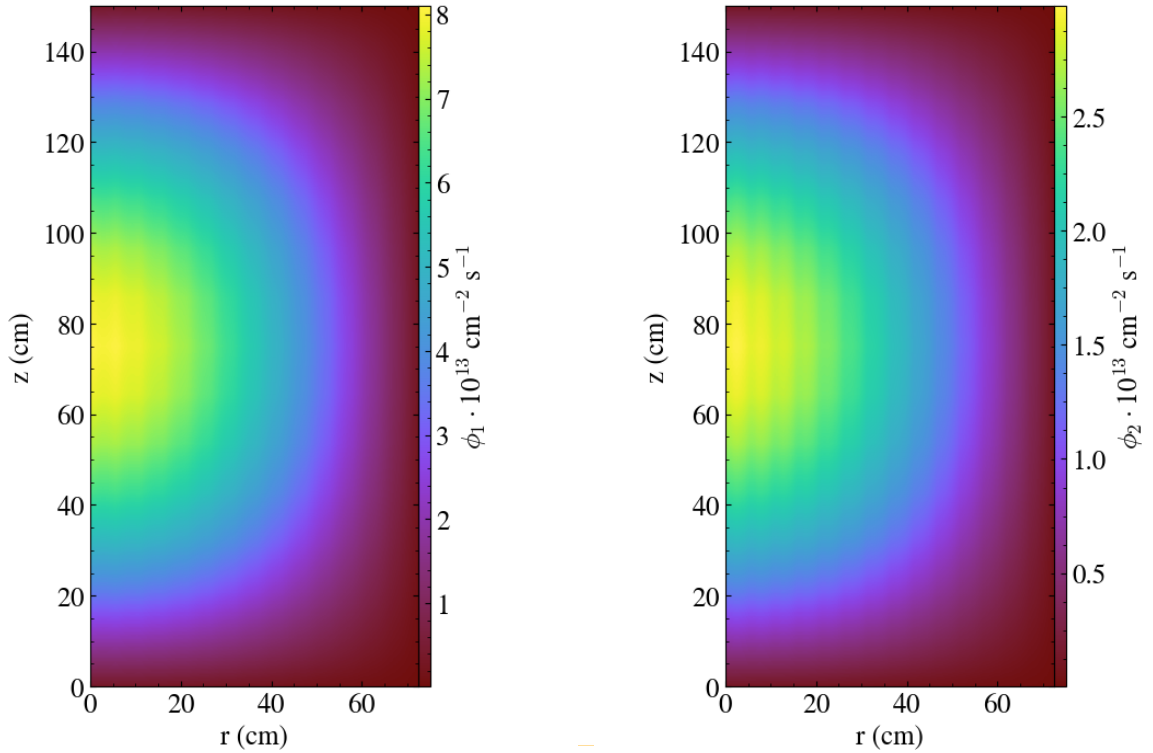
\includegraphics[height=0.85\textheight]{./images/moltres_flux.png}
   \vspace{-0.1in}
   \caption{Fast ($\phi_1$) and thermal ($\phi_2$) neutron flux obtained using Moltres 			\cite{lindsay_introduction_2018}.}
    \end{figure}
\end{frame}

\begin{frame}
  \frametitle{Multiphysics simulation results (2D) (2)}
  \begin{figure}[t]
   \vspace{-0.05in}
   \hspace*{-0.15in}
   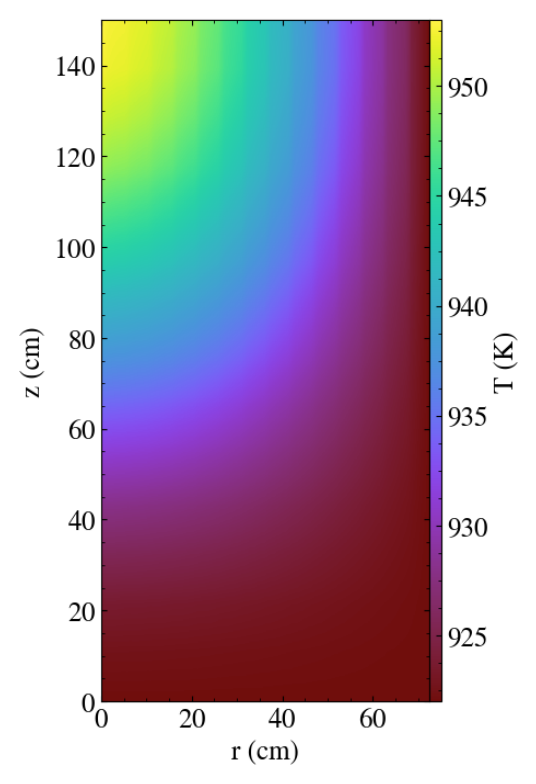
\includegraphics[height=0.85\textheight]{./images/moltres_temp.png}
   \vspace{-0.1in}
   \caption{Temperature in channel obtained using Moltres \cite{lindsay_introduction_2018}.}
    \end{figure}

\end{frame}

\begin{frame}
  \frametitle{Multiphysics simulation results (3D)}
  \begin{figure}[t]
   \vspace{-0.1in}
   \hspace*{-0.45in}
   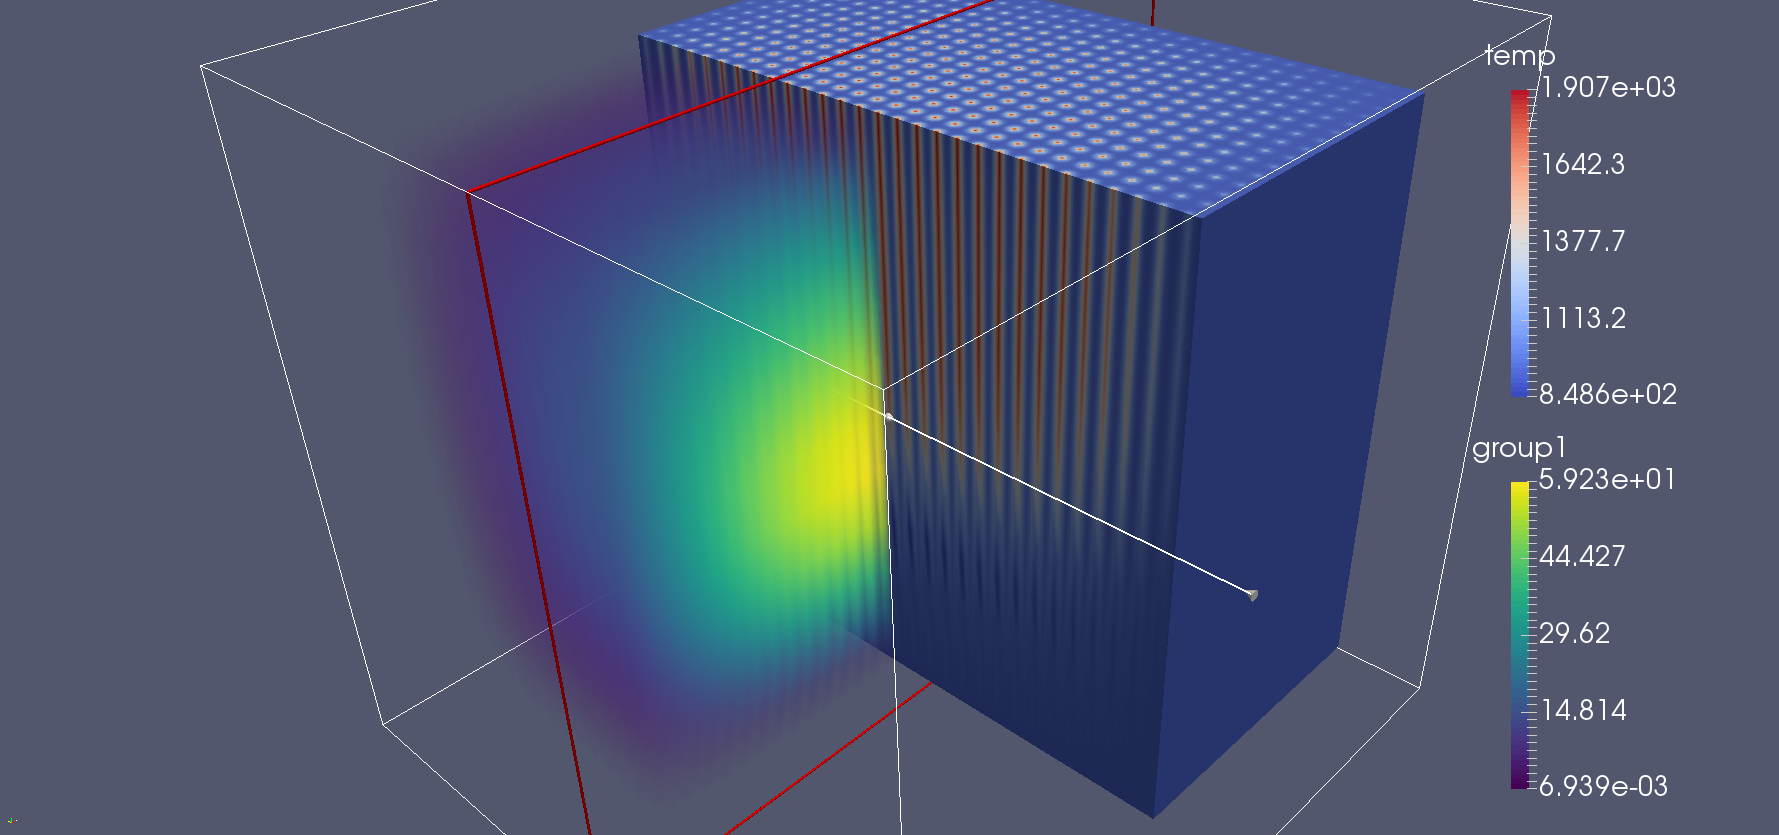
\includegraphics[height=0.75\textheight]{./images/moltres_3D.png}
   \caption{Cuboidal \gls{MSR} steady-state temperature and fast neutron flux \cite{ridley_moltres_2017}.}
    \end{figure}

\end{frame}
